\section{Introduction}

\begin{frame}{\insertsection}{Motivation}
    \begin{itemize}
        \item Query based search of documents
        \begin{itemize}
            \item Google Scholar
        \end{itemize}
        \item Encourage abstractions of underlying topics
        \begin{itemize}
            \item Rather than word frequency
        \end{itemize}
    \end{itemize}
\end{frame}

%\begin{frame}{\insertsection}{Dataset}
%    \begin{itemize}
%        \item Nordjyske news articles 2017
%        \item $\approx 63,000$ articles
%        \item Average length 231 words
%        \begin{itemize}
%            \item Spanning from 2 - 3209
%        \end{itemize}
%        \item<2-> Find a better way to search / filter these articles
%        \item<3-> Information Retrieval
%        \begin{itemize}
%            \item<4-> Ranking of document based on queries
%            \item<5-> Encourage abstractions of topics
%        \end{itemize}
%    \end{itemize}
%\end{frame}

%\begin{frame}{Preprocessing}
%    \begin{itemize}
%        \item Article Extraction
%        \only<2>{
%        \begin{itemize}
%            \item search .xml documents for text
%        \end{itemize}
%        }
%        \item Initial Document Filtering
%        \only<3>{
%        \begin{itemize}
%            \item Duplicates removed
%            \item Non-alphabetic symbols removed
%            \item Short documents removed
%        \end{itemize}
%        }
%        \item Stop Word and Word Frequency Filtering
%        \only<4>{
%        \begin{itemize}
%            \item Stop words
%            \item Rare words removed
%            \item Too common words removed
%        \end{itemize}
%        }
%        \item Word Database Filtering
%        \only<5>{
%        \begin{itemize}
%            \item Similar effect to POS-tagging
%            \item Words not in database are removed
%        \end{itemize}
%        }
%        \item Lemmatization
%    \end{itemize}
%\end{frame}

\section{Information Retrieval Methods}

%part

\begin{frame}{\insertsection}
    \begin{itemize}
        \item Latent Dirichlet Allocation (LDA)
        \item PageRank (PR)
        \item Language Model (LM)
        \item Term Frequency - Inverse Document Frequency (TF-IDF)
        \item Best Match 25 (BM25)
    \end{itemize}
\end{frame}

\subsection{Latent Dirichlet Allocation}
\begin{frame}{\insertsubsection}{Motivation}
    %Produce a generative process with the best possible chance of reconstructing the existing documents, using topics.
    \begin{itemize}
        \item Create a generative process to produce documents, based on topics
        \item Fine-tune to maximize probability of generating the original documents
        \item Use generated topics for calculating similarity
    \end{itemize}
\end{frame}

\begin{frame}{\insertsubsection}{Plate Notation}
    \begin{figure}
        \centering
        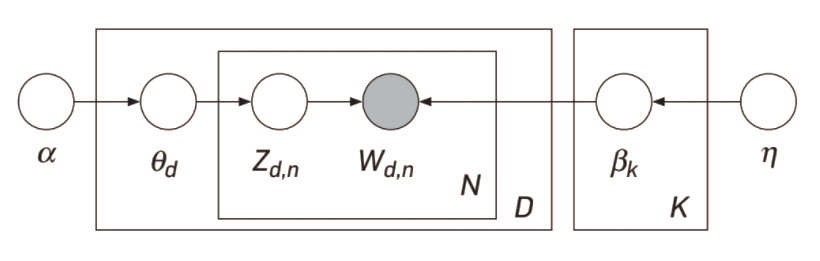
\includegraphics[width = 1 \textwidth]{figures/lda_model.jpg}
    \end{figure}
    \begin{itemize}
        \item $\alpha, \eta$ dirichlet distributions
        \item $\theta, \beta$ multinomial distributions
        \item $Z, W$ sampled topics and words
    \end{itemize}
\end{frame}

\begin{frame}{\insertsubsection}{Dirichlet Distributions}
    \begin{figure}
        \centering
        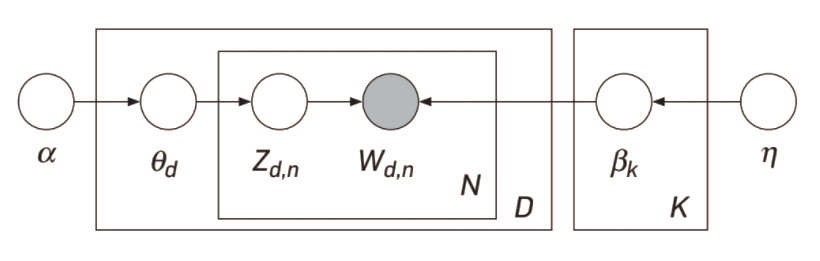
\includegraphics[width = 0.65 \textwidth]{figures/lda_model.jpg}
    \end{figure}
    \begin{figure}
        \centering
        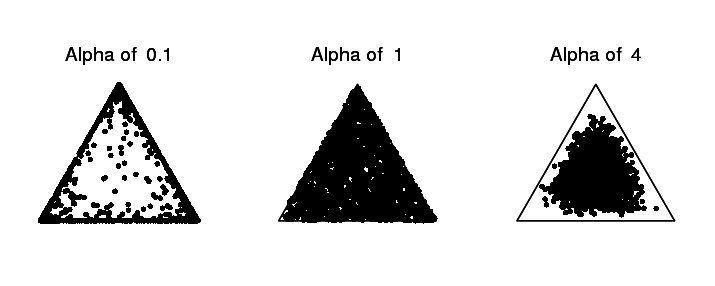
\includegraphics[width = 0.65 \textwidth]{figures/dirich.png}
        \footnote{\url{https://mollermara.com/blog/lda/}}
    \end{figure}
    \begin{itemize}
        \item<2> typical sample based on low alpha = $\{1,0,0\}$
        \item<2> typical sample based on high alpha = $\{0.333, 0.333, 0.333\}$
    \end{itemize}
\end{frame}

\begin{frame}{\insertsubsection}{Multinomial Distributions}
    \begin{figure}
        \centering
        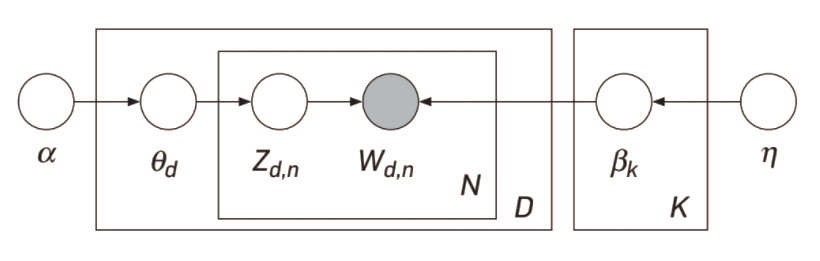
\includegraphics[width = 0.65 \textwidth]{figures/lda_model.jpg}
    \end{figure}
    \begin{itemize}
        \item Sample $N$ topics ($Z$) based on $\theta$
        \item Sample $N$ words ($W$) based on $Z$ and $\beta$
    \end{itemize}
\end{frame}

\begin{frame}{\insertsubsection}{Generation Probability}
    \begin{align*}
        & P(W,Z,\theta,\beta;\alpha,\eta) = \\
        & \prod_{d=1}^{D}P(\theta_d;\alpha)
        \prod_{k=1}^{K}P(\beta_k;\eta)
        \prod_{n=1}^{N}P(Z_{d,n}|\theta_d) P(W_{d,n}|\beta, Z_{d,n})
    \end{align*}
\end{frame}

% full example?
% training?

\subsection{PageRank}
\begin{frame}{\insertsubsection}{Overview}
    \begin{itemize}
        \item Used to rank nodes in a graph
        \item Underlying assumption: important nodes have in-going connections from other important nodes
        \item Based on the 'random surfer' model
    \end{itemize}
    \only<2>{\begin{figure}
        \centering
        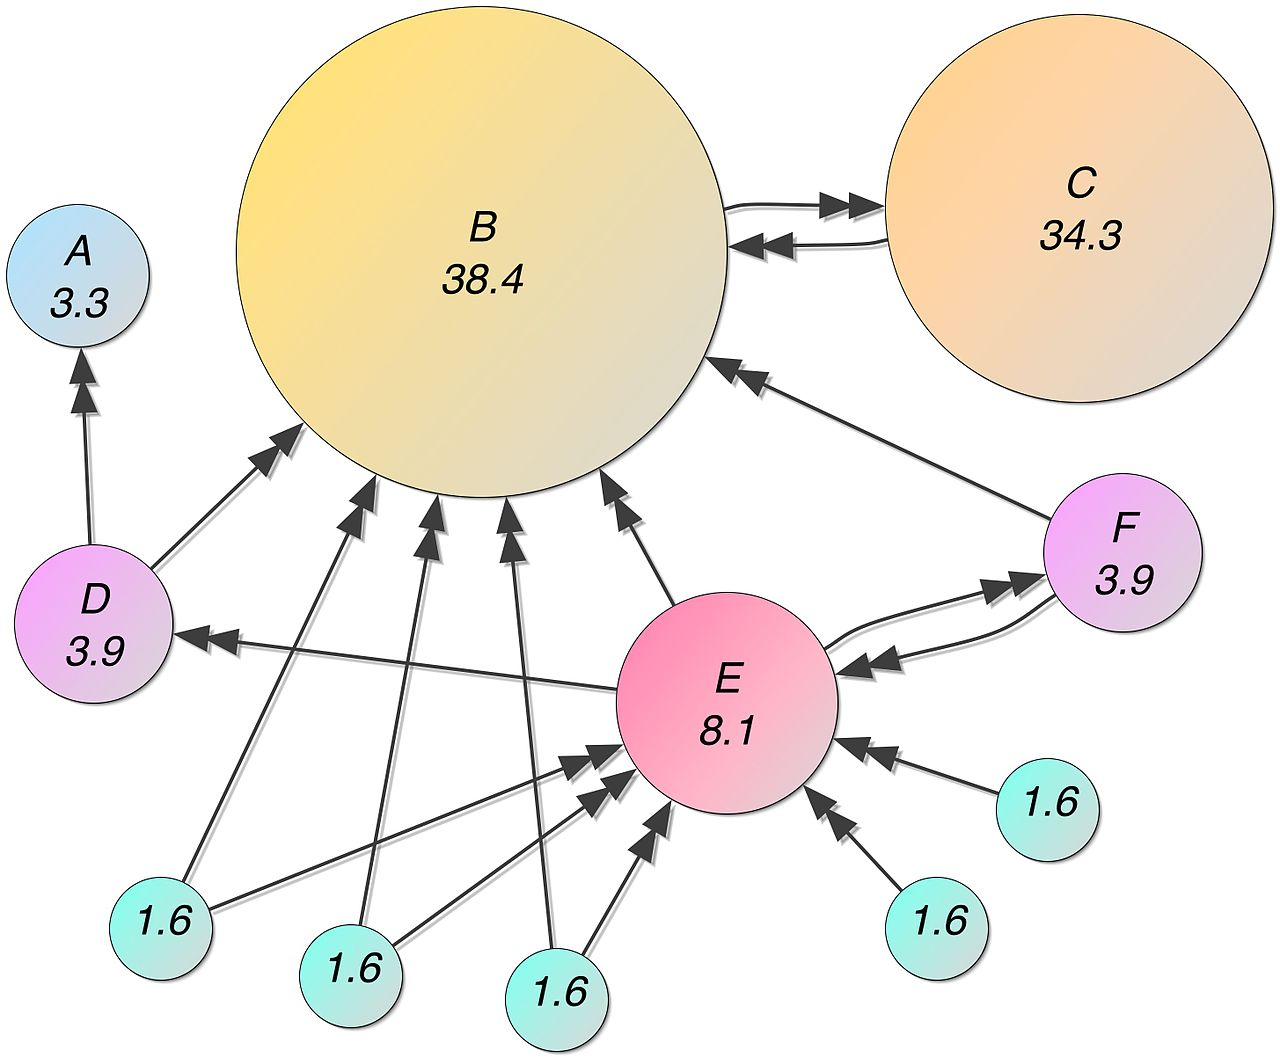
\includegraphics[width = 0.5 \textwidth]{figures/PageRank.jpg}
        \footnote{\url{https://en.wikipedia.org/wiki/PageRank}}
    \end{figure}}
\end{frame}


\begin{frame}{\insertsubsection}{Graph Construction}
    \begin{itemize}
        \item Used on adjacency matrix
        \item Similarity between documents based on $\theta$
        \begin{itemize}
                    \item Calculated using Jensen-Shannon similarity
        \end{itemize}
        \item While fully connected each edge has a value which will influence the ranking
    \end{itemize}
\end{frame}